\documentclass[12pt]{article}

\usepackage{polski}
\usepackage[utf8]{inputenc}

\usepackage{amsmath}
\usepackage{float}

% breake table between multiple pages
\usepackage{longtable}

% always add indent
\usepackage{indentfirst}

% turn on hyperlinks to the bibliography when \cite{}
\usepackage{hyperref}

% allow usage of numer set sign
\usepackage{amsfonts}

% allow usage of math signs (less than equal etc.)
\usepackage{amssymb}

% set margins
\usepackage{geometry}
\newgeometry{tmargin=2.5cm, bmargin=2.5cm, lmargin=3.5cm, rmargin=1.5cm}

% set spacing (to set '1.5' insert '1.3')
\linespread{1.3}

% add a dot after any section number
\usepackage{titlesec}
\titlelabel{\thetitle.\quad}

% center table caption
\usepackage[justification=centering]{caption}

% allow adding images
\usepackage{graphicx}
\graphicspath{ {./img/} }

\begin{document}

% set size of font in section and subsection
% \Large -> 17.28 pt (the closest to 16 pt)
% \large -> 14.4 pt (the closest to 14 pt)
\titleformat*{\section}{\Large\bfseries}
\titleformat*{\subsection}{\large\bfseries}

% add table of contents
\tableofcontents
\newpage

\section{Drzewa decyzyjne}
Drzewo decyzyjne (ang. decision tree) to rodzaj algorytmu uczenia maszynowego
wykorzystywanego do m.in. klasyfikacji danych. Na podstawie danych wejściowych budowany jest model,
który pozwala na podejmowanie decyzji. Drzewo decyzyjne przedstawiane jest graficznie jako
struktura zbudowana z węzłów, gałęzi i liści. Każdy węzeł reprezentuje test, na podstawie
którego algorytm podejmuje decyzję. Gałęzie symbolizują możliwe wyniki testu. Ostateczne
decyzje, które mogą zostać podjęte przez algorytm, reprezentowane są przez liście.

Z matematycznego punktu widzenia drzewo decyzyjne to acykliczny graf skierowany.
Gałęzie odpowiadają krawędziom grafu. Wierzchołki grafu nazywane są węzłami. Węzły, które
nie mają żadnych potomków, określane są liśćmi, natomiast węzeł nieposiadający rodzica,
nazywany jest korzeniem \cite{algorytmy-do-konstruowania-drzew-decyzyjnych}.

\subsection{Definicje}
Rekord (inaczej nazywany krotką, wierszem lub obiektem) jest wektorem wartości atrybutów.
Zbiór $n$ atrybutów wejściowych oznaczany jest przez $A = \{a_1, ..., a_i, ..., a_n\}$.
Atrybut $a_i$ przyjmuje wartości, których zbiór oznaczany jest przez
$dom(a_i) = \{v_{i,1}, v_{i,2}, ..., v_{i,|dom(a_i)|}\}$,
gdzie $|dom(a_i)|$ oznacza moc zbioru wartości atrybutu $a_i$. Atrybut wyjściowy nazywany
jest decyzją i oznaczany jest przez $y$. Możliwe wartości decyzji $dom(y) = \{c_1, ..., c_{|dom(y)|}\}$
nazywane są klasami decyzyjnymi. Przestrzeń rekordów wyznaczona jest jako iloczyn kartezjański
wszystkich zbiorów atrybutów wejściowych $X = dom(a_1) \times ... \times dom(a_i) \times ... \times dom(a_n)$
oraz zbioru atrybutów wyjściowych $dom(y)$ i oznaczana jest literą $U = X \times dom(y)$.

Zbiór treningowy $S$ to zbiór $m$ par takich, że $S = (\langle x_1, y_1\rangle, ..., \langle x_m, y_m\rangle)$,
gdzie: $m \in \mathbb{N} $, $x_q \in X$, $y_q \in dom(y)$. Zbiór $S$ graficznie przedstawiany jest jako tabela
i nazywany jest tabelą decyzyjną. Rekordy tworzą wiersze tabeli a kolumny grupują wartości atrybutów.

\begin{table}[H]
    \centering
    $\begin{array}{|c|c|c|c|}
        \hline 
        a_1 & a_2 & a_3 & y \\
        \hline \hline
        v_{1,1} & v_{2,1} & v_{3,1} & c_1 \\
        v_{1,2} & v_{2,1} & v_{3,2} & c_3 \\
        v_{1,1} & v_{2,1} & v_{3,1} & c_1 \\
        v_{1,2} & v_{2,1} & v_{3,3} & c_3 \\
        v_{1,2} & v_{2,2} & v_{3,4} & c_2 \\
        \hline
    \end{array}$
    \caption{\label{tab:decision-table}Tabela decyzyjna dla $m=5$, $|dom(y)|=3$,\\ $|dom(a_1)|=2$, $|dom(a_2)|=2$, $|dom(a_3)|=4$ i $n=3$.}
\end{table}

Selekcja $(\sigma)$ względem atrybutów przedstawiona jest za pomocą notacji używanej w algebrze.
Przykładowo wybranie z Tabeli \ref{tab:decision-table} rekordów, które dla atrybutu $a_3$ przyjmują
wartość~$v_{3,1}$, opisywane jest wyrażaniem $\sigma_{a_3=v_{3,1}}S$.

Testem $t$ nazywany jest warunek dla podziału danych. W celu wyznaczenia najlepszego testu wykorzystywane
są różne kryteria podziału.

Na podstawie tabeli decyzyjnej przy użyciu testów na atrybutach konstruowane jest drzewo decyzyjne $DT$.
Klasyfikator, który został stworzony ze zbioru treningowego $S$ oznaczany jest jako $DT(S)$. Korzystając z klasyfikatora
$DT(S)$ możliwe jest wyznaczenie predykcji $DT(S)(x_q)$ dla wybranego elementu $x_q \in X$. Rozmiar drzewa decyzyjnego $DT(S)$ oraz dokładność predykcji $DT(S)(x_q)$
w dużym stopniu zależy od wielkości zbioru treningowego $S$. Jeśli zbiór treningowy jest zbyt mały, to dokładność predykcji będzie niska.

Błąd klasyfikacji drzewa $DT(S)$ jest prawdopodobieństwem błędnej predykcji obiektu wybranego z zgodnie z rozkładem $D$ przestrzeni
etykietowanych instancji. Błąd $\varepsilon$ zdefiniowany jest następująco (w przypadku atrybutów ciągłych znak sumy zastąpowany jest całką):

\begin{equation}
    \varepsilon(DT(S), D) = \displaystyle\sum_{\langle x, y\rangle \in U} D(x, y) \cdot L(y, DT(S)(x)),
\end{equation}
\begin{equation}
    L(y, DT(S)(x)) = \left\{
        \begin{array}{ll}
            1, & DT(S)(x) = y, \\
            0, & DT(S)(x) \neq y.
        \end{array} \right.
\end{equation}

Dokładność klasyfikacji drzewa decyzyjnego obliczna jest jako $1 - L(y, DT(S)(x))$.
Rzeczywista wartość błędu klasyfikacji jest rzadko wyznaczana, ponieważ najczęściej rozkład $D$ nie jest znany.
W zamian, jako oszacowanie błędu klasyfikacji, korzysta się z błędu
obliczanego na zbiorze treningowym:

\begin{equation}
    \hat{\varepsilon}(DT(S), S) = \displaystyle\sum_{\langle x, y\rangle \in U} L(y, DT(S)(x)),
\end{equation}

Wykorzystywanie błędu wyliczanego na podstawie zbioru tr eningowego zazwyczaj daje jednak
zbyt optymistycznie oszacowanie błedu $\varepsilon$. Z tego powodu zbiór danych dzieli się na zbiór
treningowy oraz testowy. Zbiór treningowy jest większy i na jego podstawie buduje się klasyfikator.
Zbiór testowy wykorzystywany jest do wyliczania $\hat{\varepsilon}$, który zwykle zapewnia
lepsze oszacowanie błędu $\varepsilon$. 

Nadmierne dopasowanie (ang. overfitting) to sytuacja, w której utworzony klasyfikator jest zbyt
dobrze dopasowany do danych treningowych. Wystąpienie nadmiernego dopasowania sprawia, że
klasyfikator dobrze sprawdza się dla danych treningowych, jednak zmniejsza się jego zdolność
generalizacji. Oznacza to, że dla elementu $x_q$ z przestrzeni $X$, mniejsze jest prawdopodobieństwo na otrzymanie
poprawnej predykcji $DT(S)(x_q)$. W przypadku drzew decyzyjnych nadmierne dopasowanie
występuje najczęściej, gdy drzewo ma zbyt wiele węzłów w stosunku do ilości dostępnych danych treningowych.

W celu uniknięcia lub minimalizacji zajwiska nadmiernego dopasowania stosuje się technikę przycinania drzewa (ang. pruning).
Polega ona na odpowiednim upraszczaniu drzewa -- zmniejszania jego rozmiaru.
W drzewie decyzyjnym wycina się wybrane fragmenty (poddrzewa), których znaczenie jest niewielkie podczas przeprowadzania
predykcji obiektów. Poddrzewo, które zostało wybrane do wycięcia, najczęściej zastępuje się liściem z etykietą klasy, która
najczęściej występuje w wycinanym podzbiorze. Przekształcenia drzewa mogę pogorszyć dokładność klasyfikacji
na zbiorze danych treningowych, jednak często skutkują dokładniejszymi predykcjami na obiektach z poza zbioru treningowego.

\subsection{Schemat konstrukcji}
Proces budowania drzewa oparty jest na wielokrotnym podziale danych. Pierwszy krok polega na przypisaniu
korzeniowi wszystkich obiektów ze zbioru treningowego $S$. Następnie stosując wybrane kryterium podziału, które
zależne jest od użytego algorytmu, wyznaczany jest atrybut wejściowy względem którego zostanie wykonany podział obiektów.
Najlepszym podziałem jest ten, który najmniej różnicuje obiekty ze względu na ich klasę decycyjną.
Gdy wybrany zostanie atrybut, wykonywany jest test, który przydziela obiekty z węzła do nowych węzłów potomnych.
Po dopasowaniu obiektów do nowych węzłów proces podziału jest powtarzany według takiej samej zasady.
Podział powtarzny jest tak długo, aż osiągnięte zostanie kryterium stopu.

\subsubsection{Testy atrybutów}
Reguły definiujące podział w drzewach decyzyjnych są najczęściej jednowymiarowe.
Oznacza to, że test dokonywany jest na podstawie tylko jednego atrybutu.
Podziały wielowymiarowe są spotykane zdecydowanie rzadziej ze względu na złożoność obliczeniową \cite{eksploracja-danych}.
Testy podziału dzieli się w zależności od rodzaju atrybutów:

\begin{itemize}

    \item dla atrybutów dyskretnych:
    \begin{itemize}
        \item podział oparty na wartościach atrybutu:
            $$t(x) = a_i(x),$$
            gdzie:\\
            $x \in X$,

        \item podział oparty na równości:
            $$  t(x) = \left\{
                \begin{array}{ll}
                1, & \textnormal{gdy } a_i(x) = v_{i,j} \\
                0, & \textnormal{w przeciwnym wypadku,}
                \end{array} \right.
            $$
            gdzie:\\
            $v_{ij} \in dom(a_i)$,
    \end{itemize}

    \item dla atrybutów ciągłych:
    \begin{itemize}
        \item podział oparty na nierównościach:
            $$  t(x) = \left\{
                \begin{array}{ll}
                1, & \textnormal{gdy } a_i(x) \leqslant p \\
                0, & \textnormal{w przeciwnym wypadku,}
                \end{array} \right.
            $$
            gdzie:\\
            $p \in y$ (wartość progowa, cięcie),\\

        \item podział oparty na przedziałach:
            $$  t(x) = \left\{
                \begin{array}{ll}
                1, & \textnormal{gdy } a_i(x) \in I_1, \\
                2, & \textnormal{gdy } a_i(x) \in I_2, \\
                3, & \textnormal{gdy } a_i(x) \in I_3, \\
                \vdots & \\
                k, & \textnormal{gdy } a_i(x) \in I_l, \\
                
                \end{array} \right.
            $$
            gdzie:\\
            $l \in \mathbb{N}$,\\
            $I_1, I_2, I_3, ..., I_l \subset dom(a_i)$, \\
            $j \neq k \implies I_j \cap I_k = \varnothing$.
    \end{itemize}

\end{itemize}

\subsubsection{Kryteria stopu}
Faza rozbudowy drzewa trwa do momentu, gdy któryś z warunków stopu zostanie spełniony.
Wyróżnia się następujące kryteria zatrzymania konstruowania drzewa decyzyjnego:
\begin{itemize}
    \item pusty zbiór treningowy,
    \item jednorodność obiektów - wszystkie rekordy mają taką samą wartość $y$ (należą do tej samej klasy decyzyjnej),
    \item drzewo osiągnęło maksymalną wysokość,
    \item brak możliwość odnalezienia testu, który pozwoliłby na dokonanie podziału.
\end{itemize}

\subsubsection{Ocena jakości}
Dwa składowe, które wpływają na ocenę jakości drzewa decyzyjnego $Q$, to dokładność klasyfikacji oraz wielkość drzewa decyzyjnego.

\begin{equation}
Q(DT, S) = \alpha \cdot  \hat{\varepsilon}(DT(S), S) + \beta \cdot h(DT),
\end{equation}
gdzie: \\
$\alpha$, $\beta$ $\in \mathbb{R}$,\\
$h$ -- wysokość drzewa decyzyjnego.

\subsection{Algorytmy konstrukcji drzew decyzyjnych}

\subsubsection{Algorytm ID3}
Algorytm ID3 jest uważany za jeden z prostszych algorytmów konstrukcji drzew decyzyjnych.
Jako kryterium podziału wykorzystany jest zysk informacji $InformationGain$, który liczony jest
przy wykorzystaniu entropii $H$:

\begin{equation}
    H(y, S) = - \displaystyle\sum\limits_{c_j \in dom(y)}^{} \frac{\sigma_{y=c_j}S}{|S|} \cdot log_2 \frac{\sigma_{y=c_j}S}{|S|},
\end{equation}

\begin{equation}
    InformationGain(S) = H(y, S) - \displaystyle\sum\limits_{v_{ij} \in dom(a_i)}^{} \displaystyle\frac{\sigma_{a_i=v_{ij}}S}{|S|} \cdot H(y, \sigma_{a_i=v_{ij}}S).
\end{equation}

Atrybut $a_i$ dla którego zysk informacji jest najwyższy wybierany jest do wyznaczenia podziału.
Budowanie drzewa kończy się, gdy wszystkie obiekty w węźle mają taką samą wartość
klasy lub gdy najlepszy, obliczony zysk informacji nie jest większy od zera \cite{algorytmy-do-konstruowania-drzew-decyzyjnych}.

Algorytm stosowany jest dla atrybutów dyskretnych. Jeśli atrybuty są ciągłe, wówczas muszą
zostać przekształcone. ID3 nie sprawdza się w przypadku, gdy zbiór treningowy składa się z
rekordów, którym brakuje wartości pojedynczych atrybutów. ID3 jest algorytmem zachłannym,
dlatego nie daje gwarancji odnalezienia rozwiązania optymalnego, ponieważ może
utknąć w optimum lokalnym \cite{data-mining-with-decision-trees}.

\subsubsection{Algorytm C4.5}
Algorytm C4.5 jest ulepszoną wersją ID3 zaproponowaną przez tego samego autora.
Jako kryterium podziału wykorzystany został współczynnik względnego zysku informacji $GainRatio$.

\begin{equation}
    GainRatio(a_i, S) = \displaystyle\frac{InformationGain(a_i, S)}{H(a_i, S)}
\end{equation}
gdzie:\\
$k \in \mathbb{N}$, $S_k \subset S$.

W przeciwieństwie do algorytmu ID3, algorytm C4.5 może przetwarzać zarówno atrybuty dyskretne i ciągłe.
Dodatkowo jest on dostosowany do obsługi rekordów z brakującymi wartościami atrybutów. Kolejnym usprawieniem
jest zastosowanie procedury przycinania. Pozwala ona na usuwanie gałęzi wraz z połączonymi węzłami potomnymi, które
nie przyczyniają się do poprawienia dokładności klasyfikatora i zastępowanie ich jednym węzłem liścia \cite{data-mining-with-decision-trees}.


\subsubsection{Algorytm CART}
Drzewa decyzyjne skonstruowane algorytmem CART oparte są na binarnym podziale 
atrybutów. Kryterium podziału wykorzystuje indeks Giniego $Gini$, który mierzy
rozbieżności między rozkładami prawdopodobieństwa wartości atrybutów \cite{data-mining-with-decision-trees}.

\begin{equation}
    Gini(y, S) = 1 - \displaystyle\sum\limits_{c_j \in dom(y)}^{} \Bigg(\displaystyle\frac{|\sigma_{y=c_j}S|}{|S|}\Bigg)^2
\end{equation}

\begin{equation}
    GiniGain(a_i, S) = Gini(y, S) - \displaystyle\sum\limits_{v_{ij} \in dom(a_i)}^{} \displaystyle\frac{|\sigma_{a_i=v_{ij}}S|}{|S|} \cdot Gini(y, \sigma_{a_i=v_{ij}}S)
\end{equation}

Podobnie jak w algorytmie C4.5 dopuszczalne są zarówno atrybuty dysretne jak i ciągłe. Dodatkowo klasy decyzyjne
również mogą przyjmować wartości ciągłe. 

\subsubsection{Algorytm CHAID}
Algorytm CHAID (ang. Chi-squared Automatic Interaction Detectorest) to jeden z najstarszych algorytmów budowy drzew decycyjnych, który można wykorzystać 
zarówno dla atrybutów ciągłych jak i dyskretnych. Drzewa stworzone przy wykorzystaniu algorytmu~CHAID są drzewami niebinarnymi.

Dla każdego atrybutu $a_i$ znajdywana jest para wartości $\langle v_{ij}, v_{ik}\rangle$, która jest najmniej różna w odniesieniu do decyzji.
Różnica jest mierzona poprzez wykonanie testu statystycznego. Wybór testu zależy od rodzaju atrybutu wyjściowego.
Gdy jest on typu dyskretnego kryterium podziału opiera się na teście $Chi$-kwadrat. Jeśli decyzja jest typu 
ciągłego wykorzystuje się test $F$.

Dla każdej pary wartości sprawdzane jest, czy wynik testu statystycznego jest większy od progu scalania.
Jeśli wynik testu jest większy to wartości są łączone, a następnie potwarza się proces wyboru pary.
Proces jest powtarzany do momentu, gdy nie będzie możliwe odnalezienie żadnej znaczącej pary.
Następnie wybierany jest najlepszy atrybut wejściowy, który zostanie użyty do podziału bieżącego węzła,
tak aby każdy węzeł potomny składał się z grupy jednorodnych
wartości wybranego atrybutu \cite{data-mining-with-decision-trees}.

Algorytm CHAID obsługuje brakujące wartości, które traktuje jako jedna kategorie. W algorytmie nie stosuje się przycinania.

\newpage
\section{Programowanie równoległe}
Rozdział ma na celu uporządkowanie istotnych pojęć związanych z tematem programowania
równoległego. Opisane zostały podstawowe zagadnienia, różnice między programowaniem współbieżnym
i równoległym, rodzaje dekompozycji zadań, a także wzorce, stosowane w równoległych 
implementacjach algorytmów.

\subsection{Podstawowe pojęcia}
Przetwarzanie równoległe jest tematem omawianym w ramach dziedziny systemów operacyjnych.
Mimo, że celem pracy nie jest analiza zagadnień specyficznych dla systemów operacyjnych,
poniżej przestawione zostały pojęcia, których zrozumienie jest konieczne do tworzenia 
równoległych implementacji algorytmów.

\textit{Procesor} to jednostka sprzętowa, która pobiera dane z pamięci operacyjnej, interpretuje je
i wykonuje. Pojęcie procesor używane jest w dwóch kontekstach. Pierwszy, zgodny z podaną definicją, używany
jest głównie w elektronice. Drugie znaczenie procesora wykorzystywane jest częściej w programowaniu.
Wówczas pojęcie procesor jest synonimem pojęcia rdzeń.

\textit{Rdzeniem fizycznym} (ang. core) określany jest fizyczny element procesora, który pozwala na wykonywanie obliczeń.
W uproszczeniu, im więcej rdzeni posiada procesor, tym więcej obliczeń może on wykonać w jednostce czasu, co definiowane
jest jako moc obliczeniowa. Jest to jeden z czynników branych pod uwagę przy ocenie wydajności procesora. Obecnie używa się
głównie procesorów wielordzeniowych.

\textit{Rdzeń logiczny} (ang. logical core, thread) przygotowuje dane wykorzystywane podczas obliczeń wykonywanych przez rdzeń fizyczny.
Do niedawna na jeden rdzeń fizyczny przypadał jeden rdzeń logiczny.
Obecnie najczęściej każdemu rdzeniowi fizycznemu przypisuje się dwa rdzenie logiczne.
Rdzenie logiczne uzależnione są od rdzenia fizycznego, do którego są przypisane, natomiast nie są zależne
od operacji rdzeni logicznych przypisanych do innego rdzenia fizycznego.

\textit{Rozkazem} nazywane jest pojedyncze polecenie, które zapisane jest w postaci liczb binarnych i które
wykonywane jest przez procesor.

\textit{Instrukcja} definiowana jest jako bardziej złożone zadanie, które składa się ze zbioru rozkazów. Instrukcje
mogą być niskopoziomowe (napisane w np. asemblerze) lub wysokopoziomowe (napisane w np. C, Java).
Instrukcje wysokopoziomowe tłumaczone są na kilka instrukcji niskopoziomowych, natomiast instrukcje
niskopoziomowe tłumaczone są na zbiór rozkazów. Zbiór rozkazów może być dzielony na podzbiory w celu
uruchomienia każdego podzbioru na innym procesorze.

\textit{Program} jest zbiorem instrukcji, który pozwala na rozwiązanie pewnego problemu obliczeniowego. 

\textit{Proces} najprościej definiowany jest jako program, który jest w trakcie wykonywania. Pod pojęciem procesu zawiera
się jednak wiele mechanizmów, przy pomocy których system operacyjny zarządza wykonywaniem programu.
System operacyjny przydziela każdemu nowemu procesowi zasoby m.in. odrębny obszar pamięci operacyjnej, nadaje
unikatowy numer PID (process identifier), kontroluje stan procesu oraz zarządza plikami, z których korzysta proces.

\textit{Wątek} (ang. thread) jest częścią procesu. Jest to niezależny strumień instrukcji, który uruchamiany jest przez system operacyjny.
Na jeden proces najczęściej składa się wiele strumieni instrukcji. Instrukcje składające się na wątek są wykonywane sekwencyjnie.
Wszystkie wątki istniejące w ramach jednego procesu współdzielą przestrzeń adresową -- mają dostęp do pamięci wspólnej.
Z tego powodu komunikacja między wątkami należącymi do jednego procesu jest łatwa i niewymaga wsparcia systemu operacyjnego.
Przekazanie danych polega na podaniu jedynie wskaźnika do miejsca w pamięci.
Programiści często definiują wątek nieco inaczej. Wątek traktowany jest jako nieblokująca metoda, która wykonywana jest
niezależnie od procesu, który ją uruchomił \cite{programowanie-rozproszone-i-rownolegle}. Określenie wątek jest również używane
wymiennie z określeniem rdzeń logiczny. Wątek w znaczeniu rdzenia logicznego nie jest jednak równoznaczny przedstawionej definicji wątku.

\subsection{Rodzaje procesów}

\subsubsection{Proces sekwencyjny}
Proces sekwencyjny $P$ charakteryzuje się tym, że każda kolejna instrukcja $i$ wykonywana jest dopiero wtedy, gdy zakończy
się wykonywanie poprzedniej. Kolejność wykonywania instrukcji jest jednoznacznie określona, dlatego proces sekwencyjny
określany jest jako pojedynczy ciąg instrukcji \cite{wprowadzenie-do-obliczen-rownoleglych}. W przypadku procesu sekwencyjnego
wątek nie jest częścią procesu, natomiast jest z nim utożsamiany \cite{skrypt}.

\begin{figure}[H]
    \centering
	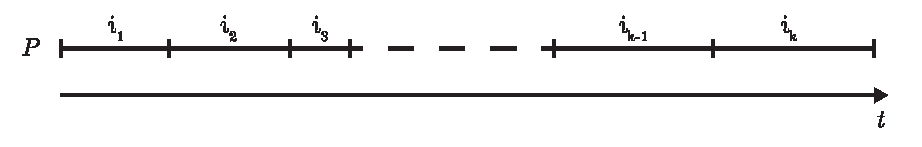
\includegraphics[width=\textwidth]{sequential.pdf}
    \caption{Proces sekwencyjny. Źródło: Opracowanie własne na podstawie \cite{wprowadzenie-do-obliczen-rownoleglych}}
    \label{fig:sequential}
\end{figure}

\subsubsection{Proces współbieżny}
Procesy sekwencyjne, które zachodzą na siebie w czasie, określane są jako proces współbieżny. Innymi słowami
proces współbieżny to proces, który składa się z wielu strumieni instrukcji.
Instrukcje należące do jednego wątku, wykonywane są, zanim ukończone zostanie wykonywanie
wszystkich instrukcji tworzących drugi, wcześniej uruchomiony wątek.

Dane są dwa procesy sekwencyjne $P_1$ i $P_2$, instrukcje $i_{1,1}, i_{1,2} \in P_1$ oraz $i_{2,1}, i_{2,2} \in P_2$.
Rysunek \ref{fig:concurrent} przedstawia jedną z wielu możliwych realizacji procesu $P_1$ oraz $P_2$.

\begin{figure}[H]
    \centering
	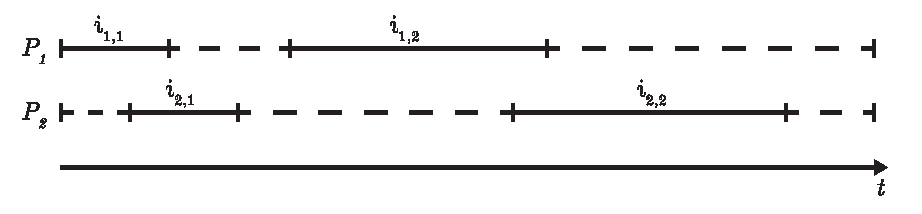
\includegraphics[width=\textwidth]{concurrent.pdf}
    \caption{Proces współbieżny. Źródło: Opracowanie własne na podstawie \cite{wprowadzenie-do-obliczen-rownoleglych}}
    \label{fig:concurrent}
\end{figure}

\subsubsection{Procesy wykonywane metodą przeplotu}
Procesy wykonywane w przeplocie są procesami współbieżnymi, w których wątki uruchamiane są naprzemiennie. Gdy wykonywany
jest proces $P_1$ to proces $P_2$ jest wstrzymywany. Gdy przerywane jest działanie procesu $P_1$ to przez pewien czas wykonywany
jest proces $P_2$. Metoda przeplotu pozwala na zastosowanie współbieżności w procesorach jednordzeniowych.

\begin{figure}[H]
    \centering
	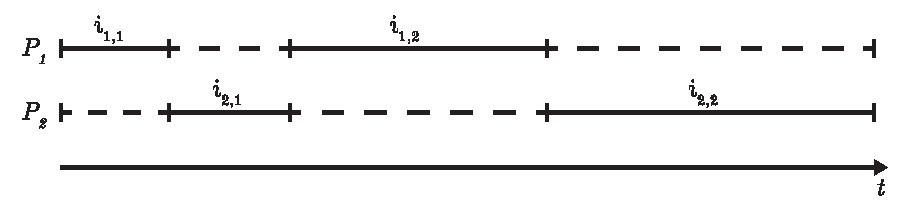
\includegraphics[width=\textwidth]{overlapping.pdf}
    \caption{Procesy wykonywane metodą przeplotu.\\ Źródło: Opracowanie własne na podstawie \cite{wprowadzenie-do-obliczen-rownoleglych}}
    \label{fig:overlapping}
\end{figure}

\subsubsection{Proces równoległy}
Proces równoległy jest szczególnym rodzajem procesu współbieżnego, w którym wątki uruchamiane są jednocześnie. Równoległe uruchamianie
wątków jest możliwe, tylko gdy wykorzystany jest specjalny sprzęt. Wątki rozdzielane mogą być między rdzenie procesora -- wtedy potrzeby
jest komputer posiadający procesor kilkurdzeniowy. Inną możliwością jest zastosowanie architektury rozproszonej. Wówczas wątki dzielone są
między zbiór komputerów, które połączone są ze sobą siecią. Proces równoległy nazywany jest wtedy rozproszonym.

\begin{figure}[H]
    \centering
	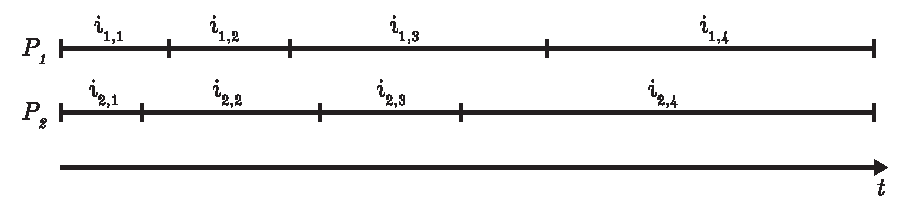
\includegraphics[width=\textwidth]{parallel.pdf}
    \caption{Procesy równoległe. Źródło: Opracowanie własne na podstawie \cite{wprowadzenie-do-obliczen-rownoleglych}}
    \label{fig:parallel}
\end{figure}

\subsection{Rodzaje dekompozycji problemów obliczeniowych}
W celu równoległego wykonywania programu istotne jest zaprojektowanie podziału zadań obliczeniowych. Podział problemu na
zadania nazywany jest dekompozycją. Wyróżniane są cztery rodzaje dekompozycji \cite{wprowadzenie-do-obliczen-rownoleglych}.

\subsubsection{Dekompozycja danych}
Dekompozycja danych to jeden z najczęściej wykorzystywanych rodzajów dekompozycji. Swoje zastosowanie znajduje szczególnie w przypadkach,
gdzie przetwarzane są bardzo duże ilości danych. Dekompozycja danych dzieli się na dekompozycję danych wejściowych i wyjściowych.
Pierwsza z nich polega na podziale danych wejściowych na względnie równe części, które przetwarzane są w ramach osobnych zadań. Najczęściej
zadania polegają na wykonaniu dokładnie takiego samego rodzaju obliczeń. Taki rodzaj dekompozycji charakteryzuje się tym,
że po zakończeniu zadań, konieczne jest ich zsumowanie.

Dekompozycja danych wyjściowych jest możliwa, gdy elementy danych wyjściowych mogą zostać wyznaczone niezależnie od siebie.
Wówczas każdemu zadaniu przydzielone zostają te dane wejściowe, które konieczne są do otrzymania poszczególnych elementów
danych wyjściowych. Wadą takiego podejścia jest stosunkowo niski stopień współbieżności \cite{wprowadzenie-do-obliczen-rownoleglych}.

Model, w którym zrównoleglanie osiągane jest poprzez zastosowanie dekompozycji danych, to model określany jest pojęciem
\textit{równoległość danych}. 

\subsubsection{Dekompozycja funkcjonalna}
Dekompozycja funkcjonalna polega na wyodrębnieniu obliczeń, których wykonanie konieczne jest do rozwiązania problemu. Obliczenia dzielone są
na grupy, które formowane są w funkcje. Zadania funkcji różnią się od siebie i najczęściej przetwarzają różne rodzaje danych
\cite{wprowadzenie-do-obliczen-rownoleglych}.
Zastosowanie dekompozycji funkcjonalnej oznacza wykorzystanie \textit{równoległości zadań}.

\subsubsection{Dekompozycja rekursywna}
Dekompozycja rekursywna stosowana jest przy rozwiązywaniu problemów metodą ,,dziel i zwyciężaj". Problem dzielony jest na
mniejsze podproblemy, które są od siebie niezależne. Każdy podproblem jest mniejszym przypadkiem pierwotnego problemu. Podział
wykonywany jest tak długo, aż podproblemy stają się trywialne do rozwiązania. Następnie wszystkie rozwiązania scalane są w jedno,
które jest ostatecznym rozwiązaniem \cite{wprowadzenie-do-obliczen-rownoleglych}.

\subsubsection{Dekompozycja eksploracyjna}
Dekompozycja eksploracyjna używana jest wtedy, gdy zadanie obliczeniowe polega na przeszukiwaniu przestrzeni rozwiązań. Przestrzeń dzielona
jest na części, które eksplorowane są równolegle przez odrębne zadania. Jeśli rozwiązanie zostanie znalezione w którejś części przestrzeni,
wówczas wykonywanie pozostałych zadań jest przerywane \cite{wprowadzenie-do-obliczen-rownoleglych}.

\subsection{Wzorce programowania równoległego}
Istnieje wiele wzorców programowania równoległego. Podczas implementacji algorytmu równoległego ciężko jest dobrać jeden, najlepiej pasujący wzorzec.
Z tego powodu wzorce traktowane są raczej jako ogólne wskazówki, które mogą być przydatne podczas projektowania algorytmu. Najczęściej programy
tworzone są zgodnie z kilkoma wzorcami, które łączone są ze sobą w celu stworzenia implementacji dopasowanej do konkretnego przypadku.
W tym rozdziale opisane zostały wybrane wzorce programowania równoległego.

\subsubsection{Wzorzec Master-Slave}
Wzorzec inaczej nazywany jest wzorcem Manager-Worker. Wątek, który nazywany jest zarządcą (Master/Manager)
definiuje zadania i rozdziela je pomiędzy wykonawców (Worker/Slave). Gdy wykonawca zrealizuje zadanie, przesyła
otrzymane wyniki zarządcy, którego zadaniem jest scalić wszystkie zgromadzone wyniki w jedno rozwiązanie problemu.
Wzorzec nie sprawdza się w problemach o dużym rozdrobnieniu zadań. Zarządca nie jest w stanie odpowiednio szybko generować
i przydzielać zadań, ponieważ wykonawcy bardzo szybko kończą realizację zadań \cite{wprowadzenie-do-obliczen-rownoleglych}.

\begin{figure}[H]
    \centering
	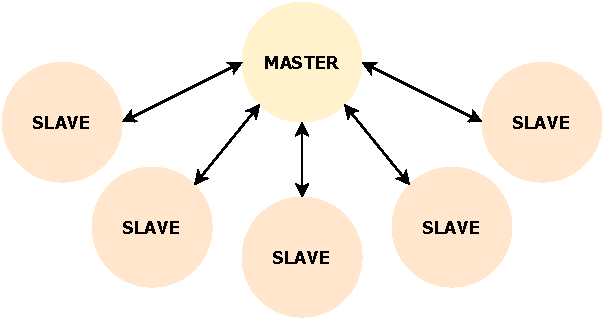
\includegraphics[width=0.5\textwidth]{patterns-master-slave.pdf}
    \caption{Wzorzec Master-Slave. Źródło: Opracowanie własne.}
    \label{fig:master-slave}
\end{figure}

\subsubsection{Wzorzec Fork-Join}
Wzorzec Fork-Join to jeden z najczęściej stosowanych wzorców. Wykonywanie programu rozpoczyna się
w ramach jeden wątku głównego. W momencie, gdy w kodzie programu pojawia się instrukcja, która wymaga
równoległego przetwarzania, tworzone są dodatkowe wątki, które wykonywane są równolegle. Dopóki wszystkie
wątki nie zakończą pracy i nie zostaną zniszczone, wątek główny nie może wznowić wykonywania
sekwencyjnej części kodu. Etap ,,fork" polega na ustawieniu argumentów, które następnie otrzymuje każdy wątek.
Etap ,,join" łączy wyniki po zakończeniu pracy wszystkich wątków równoległych. Etapy ,,fork" i ,,join"
mogę wykonywane być dowolną ilość razy. \cite{parallel-design-patterns}.

\begin{figure}[H]
    \centering
	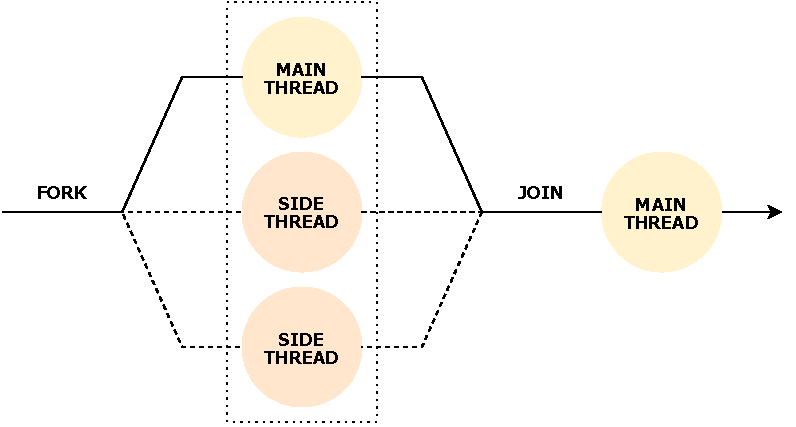
\includegraphics[width=0.6\textwidth]{patterns-fork-join.pdf}
    \caption{Wzorzec Fork-Join. Źródło: Opracowanie własne.}
    \label{fig:fork-join}
\end{figure}

\subsubsection{Wzorzec Map-Reduce}
Wzorzec Map-Reduce jest podobny do wzorca Fork-Join. Dane wejściowe są przetwarzane równolegle przez wiele wątków.
Następnie wszystkie uzyskane wyniki są łączone, aż do momentu uzyskania jednego rozwiązania.
W działaniu obydwa wzorce są prawie identycznie, jednak wywodzą się z różnych pomysłów.
Idea mapowania pochodzi z technik stosowanych w funkcjonalnych językach programowania.
Kilka mapowań może być połączonych w łańcuchy składające się na większe funkcje.
Etapy ,,map" i ,,reduce" są od siebie bardziej niezależne niż etapy ,,fork" i ,,join".
Mapowanie może występować bez redukcji, a redukcja bez mapowania~\cite{parallel-design-patterns}.

\begin{figure}[H]
    \centering
	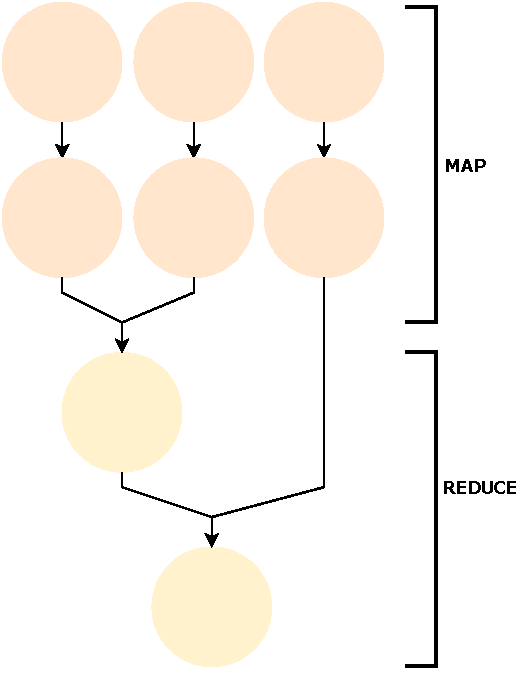
\includegraphics[width=0.4\textwidth]{patterns-map-reduce.pdf}
    \caption{Wzorzec Map-Reduce. Źródło: Opracowanie własne.}
    \label{fig:map-reduce}
\end{figure}

\subsubsection{Wzorzec Work Pool}
Wzorzec puli zadań (Work Pool) wykorzystywany jest w algorytmach, w których zadania generowane są dynamicznie
lub gdy istotnie różnią się złożonością. Zadania przechowywane są w strukturze danych, która dostępna
jest w pamięci współdzielonej. Najczęściej wykorzystywane struktury to lista, kolejka priorytetowe
czy tablica z haszowaniem. W momencie, gdy wątek zakończył obliczanie zadania, dostarczane jest mu
kolejne zadanie przechowywane w strukturze \cite{wprowadzenie-do-obliczen-rownoleglych}.

\begin{figure}[H]
    \centering
	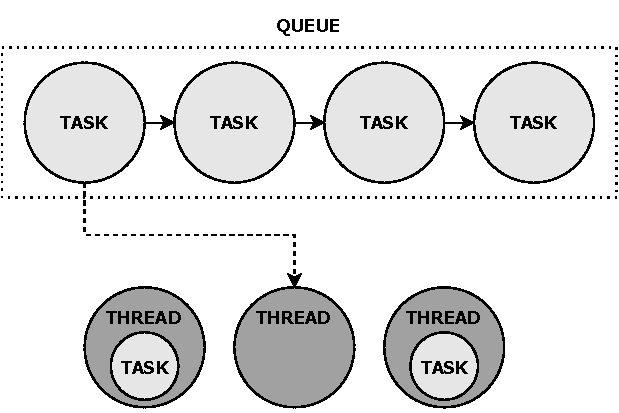
\includegraphics[width=0.55\textwidth]{patterns-work-pool.pdf}
    \caption{Wzorzec Work Pool. Źródło: Opracowanie własne.}
    \label{fig:work-pool}
\end{figure}

\subsubsection{Wzorzec Pipeline}
Wzorzec Pipeline polega na potokowym przetwarzaniu danych. Nazywany jest również metodą producenta
i konsumenta. Strumień danych przekazywany jest do kolejnych wątków, które modyfikują oryginalny strumień.
Każdy z wątków wykonuje inny rodzaj obliczeń, które tworzą etapy potoku. Dane wyjściowe jednego etapu
stają się danymi wejściowymi kolejnego etapu. Stosowanie wzorca jest efektywne, jeśli czasy realizacji
poszczególnych etapów są podobne \cite{wprowadzenie-do-obliczen-rownoleglych}.

\begin{figure}[H]
    \centering
	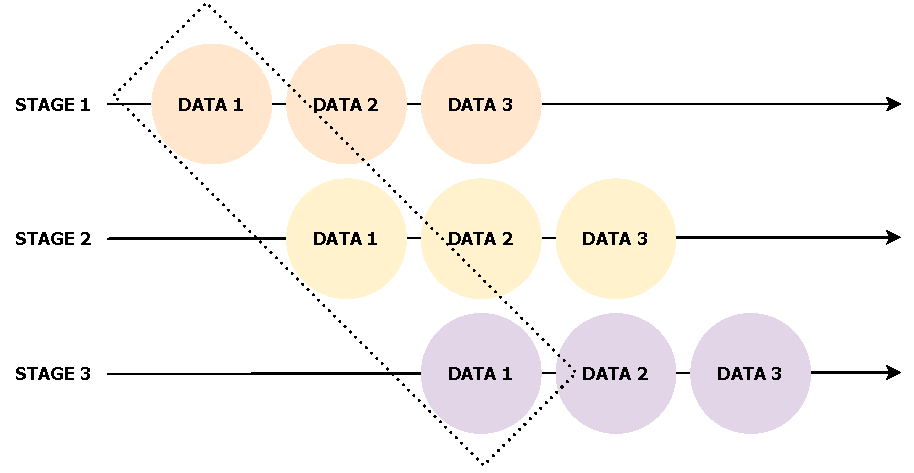
\includegraphics[width=0.75\textwidth]{patterns-pipeline.pdf}
    \caption{Wzorzec Pipeline. Źródło: Opracowanie własne.}
    \label{fig:pipeline}
\end{figure}

\newpage

\section{Przegląd literatury}

Rozdział trzeci zawiera przegląd publikacji naukowych. Tematem omawianych prac są różne metody programowania równoległego stosowane
w algorytmach uczenia maszynowego.

\subsection{Równoległe konstrukcje algorytmów drzew decyzyjnych}

W artykule \cite{parallel-implementation-decision-tree} zostało przedstawionych kilka strategii konstrukcji algorytmów drzew decyzyjnych, które oparte są o techniki takie jak: równoległość zadań,
równoległość danych oraz równoległość hybrydowa. W pracy zaprezentowana została autorska implementacja równoległej konstrukcji drzewa
decyzyjnego algorytmem C4.5. Na zakończenie autorzy przedstawili wyniki działania algorytmu i postawili wstępne wnioski dotyczące jego działania.

Artykuł rozpoczyna się od zaprezentowania trudności, które pokazują, jak złożonym zadaniem jest implementacja równoległych
algorytmów do budowy drzew decyzyjnych. Wymienione zostają m.in. problemy z zastosowaniem statycznego, jak i dynamicznego przydzielania procesorów.
Nieregularny kształt drzewa, który określany jest dopiero w momencie działania programu, jest dużą przeszkodą do stosowania statycznej alokacji. Takie podejście prowadzi
najczęściej do nierównomiernego rozłożenia obciążenia. W przeciwnej sytuacji, gdy dane przetwarzane są przez dynamicznie przydzielane procesory, problemem staje się
konieczność zaimplementowania przekazywania danych. Współdzielenie danych jest wymagane, ponieważ część danych związanych z~rodzicami musi dostępna być również dla potomków.

Autorzy szczegółowo opisują różnice pomiędzy równoległością zadań, równoległością danych oraz równoległością hybrydową. Równoległość zadań określana jest
jako dynamiczne rozdzielanie węzłów decyzyjnych między procesory, w celu kontynuowania ich rozbudowy. Wadą takiego podejścia jest konieczność replikacji całego zbioru
treningowego lub, alternatywnie, zapewnienie dużej ilości komunikacji pomiędzy procesorami. Równoległość danych przedstawiona jest jako wykonywanie tego samego zbioru instrukcji
algorytmu przez wszystkie zaangażowane procesory. Zbiór treningowy zostaje podzielony (pionowo lub poziomo) pomiędzy procesory tak, że każdy z nich odpowiedzialny jest za
inny zestaw przykładów ze zbioru. Autorzy zwracają uwagę, że przetwarzanie z pionowym podziałem danych narażone jest na~wystąpienie nierównowagi obciążenia.
Równoległość hybrydowa scharakteryzowana jest jako połączenie równoległości zadań oraz danych. Dla węzłów, które muszą przetworzyć dużą liczbę przykładów, wykorzystywana
jest równoległość danych. W ten sposób unika się problemów związanych z nierównomiernym obciążeniem. W przypadku węzłów z przypisaną mniejszą ilością przykładów
czas, potrzebny do komunikacji może być większy niż czas potrzebny do przetwarzania przykładów. Zastosowanie równoległości zadań w takie sytuacji pozwala uniknąć dysproporcji.

W kolejnej części artykułu przestawiona została implementacja równoległej konstrukcji drzewa decyzyjnego. Program został stworzony do wykonywania w środowisku pamięci
rozproszonej, w której każdy z procesorów ma~własną pamięć prywatną. Autorzy zaproponowali takie podejście, ponieważ ma ono rozwiązywać dwa problemy wspominane na
początku pracy: równoważenie obciążenia oraz konieczność przekazywania danych. Każdy z~procesorów ma za zadanie tworzyć własne listy atrybutów i klas na podstawie
przydzielonych podzbiorów przykładów. Wykorzystanie obydwu list jest kluczem do osiągnięcia efektywnego paralelizmu. Wpisy w liście klas zawierają etykietę klasy, indeks
globalny przykładu w zbiorze treningowym oraz~wskaźnik do węzła w drzewie, do którego należy dany przykład. Listy atrybutów również zawierają wpis dla każdego przykładu
z atrybutem, jak również indeks wskazujący na odpowiadający wpis w liście klas. Każdy procesor znajduje własne, najlepsze podziały lokalnego zbioru dla każdego atrybutu.
Następnie komunikuje się z pozostałymi procesorami, w celu ustalenia jednego, najlepszego podziału. Po podziale (utworzeniu węzła) następuje aktualizacja list atrybutów
przez każdy procesor, dokonana poprzez rozdzielenie atrybutów w zależności od wartości wybranego atrybutu dzielącego.

Zaprezentowane przez autorów wyniki określone są jako wstępne i wymagające udoskonaleń. Autorzy zdecydowali się jednak na wykorzystanie ich~do~przewidzenia oczekiwanego
zachowania algorytmu. Implementacja wykorzystuje takie same kryteria oceny jak stosowane w algorytmie C4.5, dlatego autorzy skupili się głównie na analizie czasu potrzebnego do
zbudowania drzewa. Do wszystkich testów wykorzystany był zestaw danych syntetycznych Agrawal, w którym każdy przykład ma dziewięć atrybutów (pięć ciągłych i~trzy dyskretne).

Z przedstawionych rezultatów testów wynika, że algorytm wykazał dobre wyniki przyspieszania. Twórcy artykułu przeprowadzili również testy mające na celu sprawdzenie skalowalności.
Jak w pierwszym przypadku, testy wykazały, że algorytm osiąga dobre wyniki skalowania.

\subsection{Równoległe uczenie zespołowe sieci neuronowych i lokalnych wzorców binarnych}

W pracy \cite{parallel-ensemble-learning} został zaprezentowany sposób pozwalający na rozpoznawanie twarzy.
Podejście oparte jest o równoległe uczenie zespołowe lokalnych wzorców binarnych (LBP) oraz konwolucyjnych sieci neuronowych (CNN). Metoda LBP zastosowana została
do ekstrakcji cech tekstury twarzy, które posłużyły jako dane treningowe sieci CNN.

Paralelizm w omawianym przykładzie został uzyskany poprzez zastosowanie równoległego uczenia zespołowego. Kilka konwolucyjnych sieci neuronowych, opartych o różne
struktury LBP, zostało wykorzystanych do uczenia się, a następnie klasyfikowania zestawów danych treningowych. Każda sieć kończyła trening podając wynik klasyfikacji. Ostateczny
wynik uzyskiwany był na podstawie głosowania większościowego. Wyjściowy wynik sieci o największej liczbie głosów przyjmowany był jako finalny klasyfikator obrazu twarzy.

W celu sprawdzenia skuteczności przedstawionego rozwiązania autorzy zdecydowali się na wybór dwóch zestawów danych: Yale-B i ORL. Zbiór Yale-B składa się 576 obrazów 38 twarzy
o różnych wyrazach, które wykonane zostały w zmiennych warunkach oświetlenia. Zbiór ORL składa się z 40 obrazów 4 twarzy, po 10 zdjęć na osobę. Współczynnik rozpoznawania
zdefiniowany został jako stosunek liczby skutecznie rozpoznanych obrazów do całkowitej ilości obrazów w zbiorze testowym. W pracy zintegrowanych zostało 10 sieci neuronowych.
Sprzęt, na którym przeprowadzono testy, posiadał następujące parametry: CPU Intel(R) Core(TM) i5-.6300HQ 2.3GHZ, pamięć RAM 8G DDR4, karta graficzna NVIDIA GeForce GTX 960M,
system operacyjny Windows 10 64 bity oraz środowisko programistyczne Python 3.5 Tensorflow-gpu 1.10.0.

Dokładność zintegrowanych sieci dla zbioru treningowego ORL wyniosła około 98\%. Po przeprowadzeniu 2800 treningów dokładność zbioru testowego zwiększyła się aż 100\%, co daje
znacznie lepszy wynik niż w przypadku zastosowania pojedynczej sieci konwolucyjnej. Dowodzi to wysokiej odporności zintegrowanych sieci na zmiany postawy ciała czy oświetlenia.
Dla zbioru Yale-B dokładność pojedynczej sieci zbliżona była do 85\%, natomiast zintegrowanej sieci wyniosła około 97,5\%. Na podstawie wyników przeprowadzonych testów
autorzy stwierdzili, że dokładność sieci neuronowej jest znacznie zmniejszona, gdy do klasyfikacji nie~wykorzystuje się schematu uczenia zespołowego.

\subsection{Równoległe implementacje algorytmu genetycznego}

Autorzy artykułu \cite{parallelized-genetic-algorithms} zaprezentowali trzy różne implementacje równoległych algorytmów gentycznych(GA):
Master-Slave, Coarse-Grained oraz Fine-Grained. Modele zostały zaimplementowane przy użyciu języka programowania Python, brokera wiadomości RabbitMQ
oraz modułu ,,Scalable Concurrent Operations in Python" (SCOOP) umożliwiającego programowanie równoległe.

W pierwszej części artykułu autorzy przedstawiają różnice pomiędzy równoległymi implementacjami a tradycyjną implementacją sekwencyjną. Model Master-Slave w wersji synchronicznej
działa prawie tak jak model sekwencyjny. Różni się tylko w przetwarzaniu funkcji Fitness, które rozdzielone jest pomiędzy różne procesory. Model Master-Slave może
zwiększyć szybkość GA poprzez równomierne rozłożenie obciążenia między procesorami, mimo konieczności komunikacji pomiędzy nimi. W modelu Fine-Grained tworzona jest jedna
globalna populacja rozproszona przestrzennie na węzły (procesory). W ten sposób zostaje utworzona topologia z sąsiedztwami. Sąsiedztwa tworzą przestrzeń, w której odbywa się równoległa i
tylko lokalna selekcja (osobnik uczestniczy w selekcji tylko w obrębie sąsiedztwa). Z powodu izolacji sąsiedztwa, najlepsze osobniki rozprzestrzeniają się wolnej niż w innych rodzajach GA,
co zwiększa różnorodność populacji. Dodatkowo tylko jeden element centralny w obrębie jednego sąsiedztwa jest poddawany modyfikacjom przez krzyżowanie i mutacje. Do zalet tego modelu
autorzy zaliczają dużą wydajność. Model Coarse-Grained różni się od modelu Fine-Grained głównie tym, że pracuje on z mniej rozdrobnioną globalną populacją (w przypadku Fine-Grained
jest to po jeden lub dwa osobniki na węzeł). Autorzy przyjmują zasadę, że model Coarse-Grained występuje wtedy, gdy liczba węzłów jest mniejsza niż liczba osobników w jednym z nich.

Paralelizacja GA została otrzymana poprzez użycie funkcji z modułu SCOOP, natomiast do komunikacji między procesami wybrany został serwer RabbitMQ. Testy pomiędzy poszczególnymi
implementacjami a implementacją szeregową zostały przeprowadzone na następującym sprzęcie: Linux z~systemem operacyjnym Fedora wersja 25, CPU Intel(R) Xeon(R) L5408
2.13 GHz z czterema procesorami, pamięć RAM 32 GB z wirtualizacją trzech innych stacji roboczych z systemem operacyjnym Ubuntu 17.10. Rozmiar populacji rozpoczynał się od
64 osobników, a następnie zwiększany był dla kolejnych testów.

Zgodnie z oczekiwaniami autorów, najmniejsze zapotrzebowanie na pamięć operacyjną wykazał model sekwencyjny. Model Coarse-Grained charakteryzował się natomiast największym
zużyciem pamięci. Pomiędzy modelami równoległymi niższym zużyciem CPU wyróżnił się model Master-Slave. Efektywność samego algorytmu oceniana jest w artykule poprzez porównanie
liczby iteracji potrzebnych do znalezienia najlepszego rozwiązania. We~wszystkich równoległych modelach GA można było zaobserwować zależność pomiędzy liczbą iteracji, wielkością
populacji oraz zużyciem pamięci. Wraz ze~wzrostem ilości osobników liczba iteracji malała, natomiast wzrastało zużycie pamięci. Najszybszym modelem okazał się model Fine-Grained,
który uzyskiwał najlepszy wynik prawie 27-krotnie szybciej niż model sekwencyjny. Testy przeprowadzone przez autorów potwierdziły korzyści płynące z wykorzystania równoległych
implementacji algorytmu genetycznego. Wszystkie trzy modele równoległe osiągnęły istotne przyspieszenie i lepszą wydajność w porównaniu z modelem sekwencyjnym. W szczególności
modele Fine-Grained i Coarse-Grained były bardziej wydajne, ponieważ liczba wymaganych iteracji była znacznie mniejsza niż w modelu sekwencyjnym.

\subsection{Zestawienie artykułów}

W literaturze można znaleźć wiele artykułów na temat metod programowania równoległego wykorzystywanego do optymalizacji pracy algorytmów uczenia maszynowego. 
Metody jednak mogą znacznie się od siebie różnić w zależności od rodzaju algorytmu, dla którego są przeznaczone. W dalszej części pracy uwaga zostanie poświęcona
już tylko podejściom stosowanym w algorytmach do budowy drzew decyzyjnych.

Tabela \ref{table:articles-parallel-decision-tree} zawiera odnośniki do tytułów artykułów, słowa kluczowe oraz krótki opis przybliżający tematykę poruszaną w każdym z artykułów.

    % \renewcommand{\arraystretch}{1.5}
    % \setlength{\tabcolsep}{0.07\textwidth}
    \begin{center}

        \begin{longtable}{| c | p{0.19\textwidth} | p{0.62\textwidth} |}

            \hline
            
            \textbf{Artykuł} &\textbf{Słowa kluczowe} & \multicolumn{1}{|c|}{\textbf{Opis}}
            
            \\ \hline \hline 

            \cite{parallelization-of-decision-tree-al} &

            równoległość wewnątrzwęzłowa; równoległość międzywęzłowa &

            Autorzy przedstawili oraz porównali wydajność czterech metod do równoległej implementacji algorytmu C4.5.
            W~analizie uwzględniony został rodzaj danych wykorzystywanych do konstrukcji drzewa, który okazał
            się mieć duży wpływ na wyniki wydajności porównywanych metod. Wyszczególnione zostały trzy rodzaje
            techniki wewnątrzwęzłowe, które wykorzystują zrównoleglanie przetwarzania danych. Równolegle
            przetwarzane mogą być rekordy, atrybuty lub ich kombinacja (podejście hybrydowe). W technice międzywęzłowej
            równolegle przetwarzane są całe węzły -- wszystkie operacje, które muszą zostać przeprowadzone do stworzenia
            węzła, wykonywane są przez jeden wątek. \\
            
            \hline

            \cite{parallel-hoeffding-decision-tree} &

            węzły Hoeffdinga; architektura Master-Slave; &

            Autorzy artykułu zdecydowali się na zrównoleglanie tylko fragmentów algorytmu tj. szukania
            najlepszego atrybuty do podziału węzła. Zadania przydzielane przez główny procesor
            (master) innym procesorom (slave) polegają na obliczenia zysku informacyjnego dla określonego
            atrybutu. Zastosowana architektura oraz zrównoleglanie tylko wyszukiwania atrybutów skutkuje
            jednak w niskiej skalowalności. Pomimo tego testy wykazały, że przyspieszenie działania algorytmu
            jest dość efektywne. Dzięki zastoso- \\
            
            & 

            &
            waniu nierówności Hoeffdinga, do podziału drzewa nie muszą być
            używane wszystkie dane. Ma to dodatkowy wpływ na szybkość działania algorytmu. \\
            
            \hline

            \cite{parallel-algorithm-to-induce-decision-trees} &

            równoległość w węźle; duże zbiory danych &

            W artykule przedstawiono algorytm ParDTLT. Algorytm jest równoległą wersją algorytmu
            DTLT (Decision Trees from Large Training sets), który nie wymaga ładowania w całości wszystkich danych
            treningowych do pamięci komputera. ParDTLT oparty jest na idei sekwencyjnej budowy struktury
            drzewa oraz równoległym przetwarzaniu danych w każdym węźle. W danym czasie wszystkie procesory
            dostępne są dla jednego węzła. W węźle uprzywilejowanym tworzona jest kolejka atrybutów, dla
            których obliczany jest zrównoważony zysk informacji. Analiza kolejnych
            atrybutów przydzielane są procesorom do momentu, aż kolejka będzie pusta. Pozostałe węzły drzewa czekają, aż
            staną się węzłem uprzywilejowanym. Autorzy artykuły przeprowadzili testy algorytmu, które wykazały, że
            ParDTLT jest szybszy od algorytmów jak np. DTLT czy C4.5. \\

            \hline

            \cite{improved-id3-decision-tree} &

            wielowątkowość; pamięć \newline współdzielona; algorytm ID3 &

            Modyfikacjom został poddany algorytm ID3. Przedstawiono dwie różne implementacje wykorzystujące równoległość.
            Pierwsza polega na stworzeniu tylu wątków, ile istnieje atrybutów, dla których obliczony musi zostać
            przyrost informacji. Gdy atrybut dzielący zostanie odnaleziony, tworzony jest węzeł. Następnie ponownie
            tworzone są kolejne wątki, które przetwarzają atrybuty nowo powstałych węzłów. Dopiero gdy wszystkie wątki
            zakończą pracę, z dostarczonych wyników składane jest drzewo. Różnica w drugiej implementacji polega na 
            wykorzystaniu pamięci współdzielonej, dzięki czemu algorytm jest bardziej wydajnym pamięciowo. 
            Węzeł główny jest współdzielony, dlatego każdy nowy węzeł może być tworzony, gdy tylko atrybut dzielący
            został odnaleziony. \\
            
            \hline

        \caption{Zestawienie artykułów poruszających tematykę\\ równoległości w algorytmach drzew decyzyjnych}
        \label{table:articles-parallel-decision-tree}
 
        \end{longtable}

    \end{center}

\listoftables
\listoffigures
\newpage

\begin{thebibliography}{20}

    \bibitem{programowanie-rozproszone-i-rownolegle} Andrzej Karbowski, Ewa Niewiadomska-Szynkiewicz. Programowanie równoległe i rozproszone. Oficyna Wydawnicza Politechniki Warszawskiej. Warszawa, 2009.
    \bibitem{wprowadzenie-do-obliczen-rownoleglych} Czech Zbigniew J. Wprowadzenie do obliczeń równoległych. Wydawnictwo Naukowe PWN. Wyd. 2, 2013.
    \bibitem{skrypt} Krzysztof Banaś, Skrypt. Programowanie równoległe i rozproszone. Wydział Fizyki, Matematyki i Informatyki Politechniki Krakowskiej. Kraków, 2011.
    \bibitem{data-mining-with-decision-trees} Lior Rokach, Oded Maimon. Data Mining with Decision Trees. Theory and Applications. World Scientific Publishing Company. Israel, 2014.
    \bibitem{parallel-design-patterns} OpenCSF Project. [Online] \url{https://w3.cs.jmu.edu/kirkpams/OpenCSF/Books/csf/html/ParallelDesign.html}. Dostęp: 12.12.2022
    \bibitem{eksploracja-danych} Dariusz Majerek. Eksploracja danych. [Online] \url{https://dax44.github.io/datamining/drzewa-decyzyjne.html#w%C4%99z%C5%82y-i-ga%C5%82%C4%99zie}. Dostęp: 02.12.2022
    \bibitem{algorytmy-do-konstruowania-drzew-decyzyjnych} Kozak J., \& Juszczuk P. (2016). Algorytmy do konstruowania drzew decyzyjnych w przewidywaniu skuteczności kampanii telemarketingowej banku. Studia Informatica Pomerania nr 1/2016 (39). doi: 10.18276/si.2016.39-05

    \bibitem{parallel-implementation-decision-tree} Amado, N., Gama, J., \& Silva, F. (2001). Parallel Implementation of Decision Tree Learning Algorithms. Lecture Notes in Computer Science, 6-13. doi:10.1007/3-540-45329-6\_4 
    \bibitem{parallel-ensemble-learning} Tang, J., Su, Q., Su, B., Fong, S., Cao, W., \& Gong, X. (2020). Parallel Ensemble Learning of Convolutional Neural Networks and Local Binary Patterns for Face Recognition. Computer Methods and Programs in Biomedicine, 105622. doi:10.1016/j.cmpb.2020.105622
    \bibitem{parallelized-genetic-algorithms} Skorpil, V., Oujezsky, V., \& Tuleja, M. (2020). Testing of Python Models of Parallelized Genetic Algorithms. 2020 43rd International Conference on Telecommunications and Signal Processing (TSP). doi:10.1109/tsp49548.2020.9163475
    \bibitem{parallelization-of-decision-tree-al} Kubota, K., Nakase, A., Sakai, H., \& Oyanagi, S. (2000). Parallelization of decision tree algorithm and its performance evaluation. Proceedings Fourth International Conference/Exhibition on High Performance Computing in the Asia-Pacific Region. doi:10.1109/hpc.2000.843500
    \bibitem{parallel-hoeffding-decision-tree} Cal, P., \& Woźniak, M. (2013). Parallel Hoeffding Decision Tree for Streaming Data. Advances in Intelligent Systems and Computing, 27-35. doi:10.1007/978-3-319-00551-5\_4
    \bibitem{parallel-algorithm-to-induce-decision-trees} Rcega, A. F.-A., Suarez-Cansino, J., \& Flores-Flores, L. G. (2013). A parallel algorithm to induce decision trees for large datasets. 2013 XXIV International Conference on Information, Communication and Automation Technologies (ICAT). doi:10.1109/icat.2013.6684045 
    \bibitem{improved-id3-decision-tree} Maheshwari, S., Jatav, VK., \& Meena, YK. (2011). Improved ID3 Decision Tree Generation using Shared-Memory and Multi-Threading Approach. 2011 International Conference on Education Technology and Computer (ICETC 2011). doi:10.13140/2.1.3216.2247

\end{thebibliography}


\end{document}